\documentclass[15pt]{standalone}
\usepackage{xcolor}
\usepackage{tikz}
\usepackage{pgfplots}
\definecolor{original}{HTML}{d5002d}
\definecolor{simple}{HTML}{03af7a}
\definecolor{approx}{HTML}{005aff}
\begin{document}
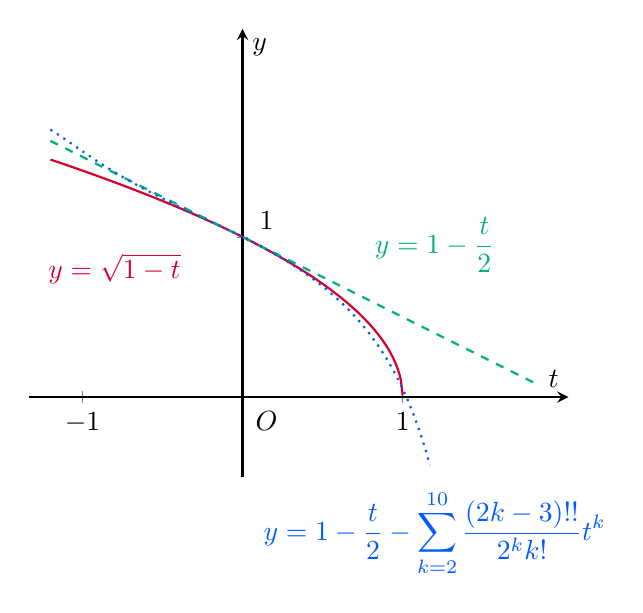
\begin{tikzpicture}
    \begin{axis}[
        axis equal,
        axis lines=middle,
        axis line style=thick,
        xlabel={$t$},
        ylabel={$y$},
        ytick={1},
        yticklabels={},
        xtick={-1, 1},
        domain=-1.5:2.3,
        xmin=-1.3,
        xmax=2,
        ymin=-0.5,
        ymax=2.3,
        samples=200,
        clip=false
    ]
    \addplot[original, thick][domain=-1.2:0.9999] {sqrt(1 - x)};
    \addplot[simple, thick, dashed][domain=-1.2:1.85] {1 - x/2};
    \addplot[approx, thick, dotted][domain=-1.2:1.17] {%
        1
        - x/2
        - x^2 / 8
        - 3 * x^3 / 16
        - 5 * x^4 / 128
        - 7 * x^5 / 256
        - 21 * x^6 / 1024
        - 33 * x^7 / 2048
        - 429 * x^8 / 32768
        - 715 * x^9 / 65536
        - 2431 * x^10 / 262144
        % - 4199 * x^11 / 524288
        % - 29393 * x^12 / 4194304
    };
    \node (O) at (axis cs:0.15, -0.15) {$O$};
    \node (one) at (axis cs:0.15, 1.1) {$1$};
    \node (original) at (axis cs:-0.8, 0.8) {\textcolor{original}{$\displaystyle y = \sqrt{1 - t}$}};
    \node (line) at (axis cs:1.2, 0.95) {\textcolor{simple}{$\displaystyle y = 1 - \frac{t}{2}$}};
    \node (lim) at (axis cs:1.2, -0.85) {\textcolor{approx}{$\displaystyle y = 1 - \frac{t}{2} - \sum_{k = 2}^{10} \frac{(2k - 3)!!}{2^k k!} t^k$}};
    \end{axis}
    \end{tikzpicture}
\end{document}
